% Chapter 3
\chapter{Achieving sustainable competitive advantage} % Main chapter title
\label{Chapter3} % For referencing the chapter elsewhere, use \ref{Chapter1} 

\lhead{Chapter 3. \emph{Achieving sustainable competitive advantage}} % This is for the header on each page - perhaps a shortened title

\setstretch{1}
%----------------------------------------------------------------------------------------

\section{Comparative analysis}
  % About Jinni's growth due to technological differentiation ... explain 
  In previous section, information about features used by companies to provide movie recommendations to users are summarized. Since the goal of this report is to compare features provided by our competitors and to understand how technological differentiation in developed product increases the possibility of achieving sustainable competitive advantage. Popularity index of a movie recommendation engine in current situation is as shown in figure \ref{fig: Popularity of competitors} , a websites popularity entirely depends on the number of unique visitors making use of the recommendation service. It becomes crucial to understand the reasons behind popularity of a particular website, this information helps in contrasting it with its competitors to know more about their success strategy in both technical and business domain. 

  On the technical front, features related to the core product, in our case movie recommendation engines are compared by using datum obtained during literature survey. A interesting metric for a website to be more intriguing to the user is time spent by an average user in viewing the content, the graph in figure \ref{fig: Time Spent by an average user} displays this information. A noticeable observation in this graph is about time spent by an average user in Jinni website, despite of it being a new company compared to \acrshort{IMDB} there is a high viewing time by visitors. The reason is that Jinni has innovative features not limited to mood based recommendations, user friendly interface and easy import of rating data from other recommendation websites. More about features that are essential for a recommender website to gain popularity are compared in following subsection \ref{Comparision_of_features} and comparing Vionel's planned features with features provided by state of the art recommender engine in current market in subsection \ref{Comparision_with_state_of_the_art}.        

 \subsection{Comparison of features}  
 \label{Comparision_of_features}
  
   \begin{figure}[htbp]
	\centering
		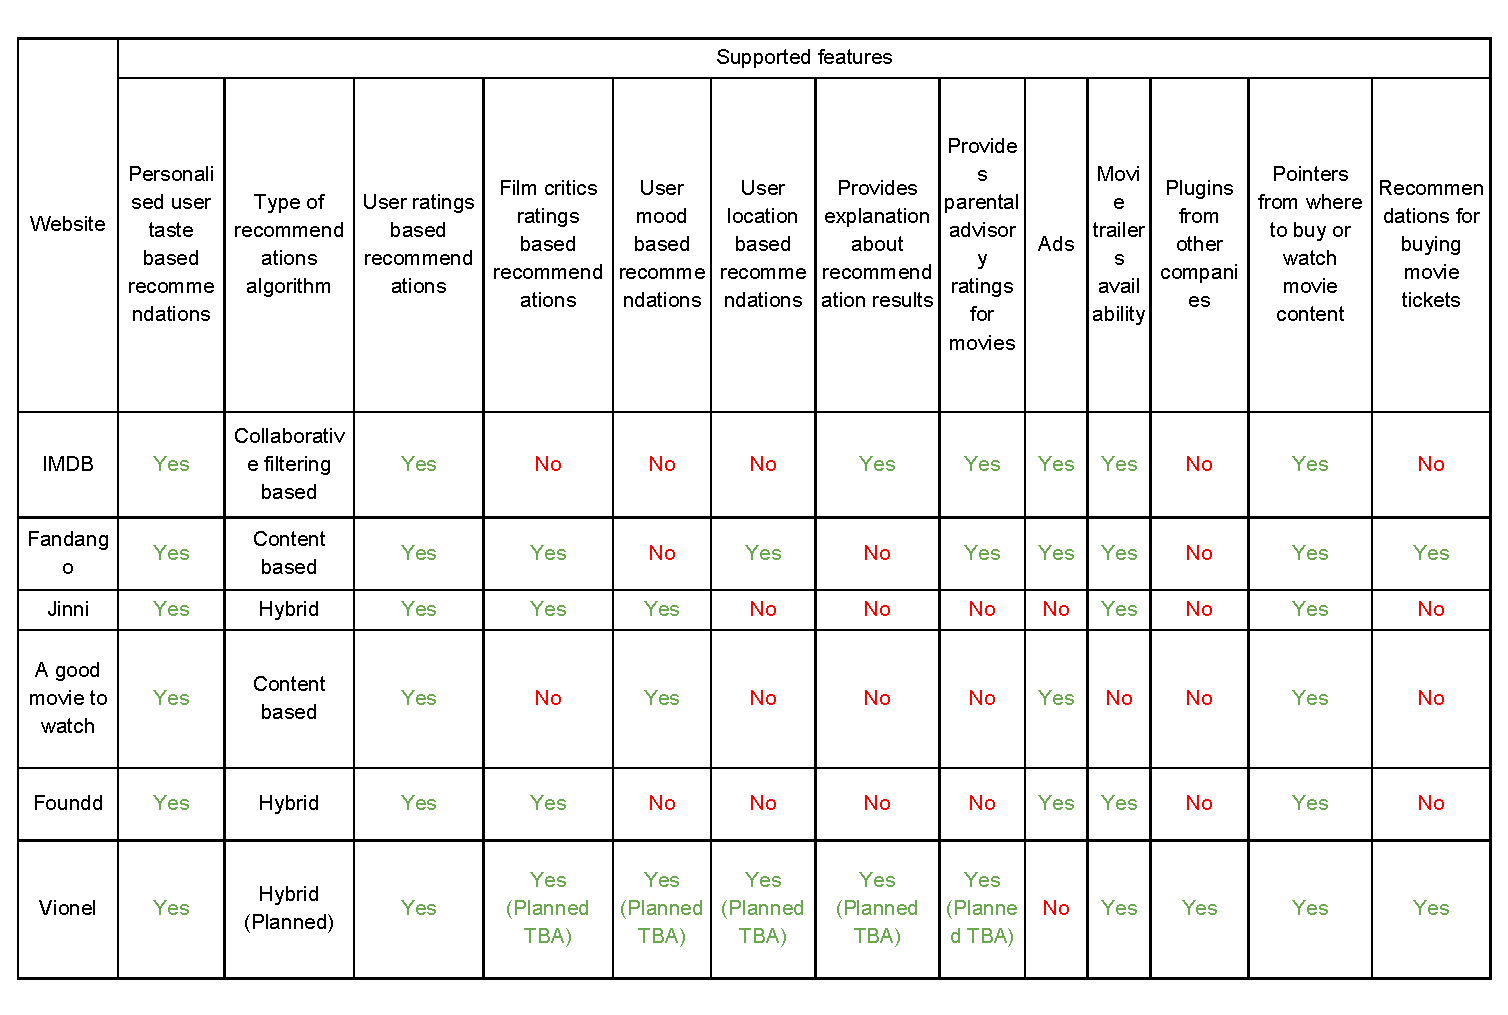
\includegraphics[scale=0.6]{Figures/Features_comparison.pdf}
		%\rule{35em}{0.5pt}
	\caption[Table : Summarized feature comparison table]{ Summarized feature comparison table}
	\label{Table: Feature comparison}
   \end{figure}
    
   As shown in the table \ref{Table: Feature comparison}, the distinctive features of movie recommendation engines are tabulated in order to enable faster comparison of features provided by each website. By comparing features provided along with the information of popularity of websites, provides clue for which feature is crucial for a website to be popular among users. Our fierce competitor \acrshort{IMDB} has a large fan base, the reason for its popularity is sheer amount of movie information it contents. In spite of attracting more number of users, \acrshort{IMDB} is unsuccessful to engage users for longer duration in website. Whereas, a recent innovative startup from Israel, Jinni is able to retain users for longer duration of time. The reason for Jinni to be so engaging is provision for users to search for movies in an innovative way based on mood information and also based on other innovative tag category for movies. Most of the older recommendation engines either use content based or collaborative filtering based recommendation algorithms. The algorithm should use both user ratings and film critics ratings for generating recommendations. Websites that only use user's rating based recommendations have a danger of suggesting irrelevant movies to the user, if the collected rating information for a movie is corrupted deliberately by users. Hence, Vionel is planning to use both user ratings and film critic ratings to generate recommendations. New startups such as Foundd, Jinni have a combination of both content based and collaborative filtering based algorithms to better match taste of the user. An innovative feature of providing information about the type of content in the movie is part of \acrshort{IMDB} and Fandango's website, which is a better feature to have parental advisory control for display of movie content. A company Fandango provides content based recommendations, along with this it provides users with a suggestive list of links from where movie tickets can be purchased. This feature has made this website quite popular and it has become a goto location for all movie enthusiasts in USA. Vionel has already adopted its architecture to suggest users with the information of availability of movie content.  

   Advertisement free environment is appreciated by users of the website, on the other hand users enjoy availability of plug-ins from other companies containing songs from movies and trailers, in movie information catalogue. Hence it is planned to support these features which are popular among users to Vionel website, in order to attract more users. Also on top of this there is a need to innovate and add other features related to recommendations, more information about adding new technical features and how these features help in attaining competitive advantage are discussed in subsection \ref{Technical_changes_to_increase_uniqueness}.  

 \subsection{Comparison with state of the art}
 \label{Comparision_with_state_of_the_art}
 % compare and write the same thing , tech , biz etc
 The task of competitor analysis is to understand the factors that enabled a competitor to succeed, and use this knowledge to improve the condition of current product. In movie recommendations, \acrshort{IMDB} is undoubtedly the state of the art in terms of availability of movie content and also quality of recommendations provided. The backbone of recommendations is based on user's movie rating data, and \acrshort{IMDB} has collected this information from past decade to become a largest movie information database. In order to compete, Vionel has to collect more user data, and also movie information by creating ties with movie production franchises and companies that have user data related to entertainment. 

 Interesting and distinctive features from all of the competitors are used as guiding light to build our recommendation system. An example of this is \acrshort{IMDB} has a large database, but uses collaborative filtering for suggesting movies to the user. Whereas it is planned to use both content and collaborative filtering in providing suggestions for users in Vionel. The feature of providing mood based recommendations are obtained from Jinni and company named ``A good movie to watch''. Since people like to receive recommendations based on mood and to find a not so popular movie with great subject to watch. In order to out rank the state of the art competitor, few features of an ideal recommendation engine as described in \ref{State of the art movie recommendation engine}, are planned to be included in Vionel. The features related to computer vision and machine learning are used to improve the current state of the recommendation engines. 
 
\section{Challenges for attaining competitive edge}
 % Challenge explanation,  
  Vionel faces challenges on both technical and business front. The challenges faced by Vionel in technical side are concerned with improving accuracy of recommendations, inclusion of new features by researching in the domain of computer vision and machine learning. The challenge of solving the problem of cold start in the case of recommendation engines. One more important aspect is about privacy issues related to usage of users private information, hence a challenge for Vionel is to provide quality recommendations by respecting user's privacy levels. Overall, Vionel is facing the challenge of being unique by innovating and creating a technical differentiation from its competitors.

  On the business front there is need for partnering with companies, to enable addition of innovative features. Also there is a challenge in creating a barrier to new entrants in the domain of movie recommendation engines. The solution for solving technical and business related challenges are discussed in further sections.     

\section{Changes needed to face the challenge}
 \label{Changes_needed_to_face_the_challenge}
 % tech,block diagram explanation , biz
 For a technology based startup like Vionel, the best way of attaining competitive edge is by introducing innovative features into their products. In order to enhance customer experience and increase the number of visitors, Vionel's \acrshort{MRS} should make use of innovative movie data analysis techniques to improve quality of recommendations provided to the user. To face the challenge changes has to be made in both technical and business front. Inclusion of few innovative features requires few business oriented changes such as partnering with complementers, suppliers and other companies that provide required data. The following subsections \ref{Buisness_related_changes} and \ref{Technical_changes_to_increase_uniqueness} explains about the steps that have been either initiated or planned to be incorporated in near future by marketing and R\&D team of the company respectively. The information about planned activity is collected from discussion with respective members of the team. All the changes are planned by objective of enhancing user's experience and to encourage more number of users to use Vionel's recommendation engines.

 % Spotify 
 \subsection {Business related changes} 
  \label{Buisness_related_changes} 
    Movie recommendations are as good as the database of movie information available at recommender algorithm's disposal. In order to improve the quality of recommendations, it is essential to add information about movies from all over the world. Currently, it has been planned to use open source movie databases to facilitate recommendations. Even though a complementer to our product such as Warner Bros., a movie production company, has ties with Vionel. To avail even more reliable movie meta-data, there is a need for building strong ties with other popular movie production agencies such as 20th century fox, Castle rocks entertainment, Marvel studios and many other complementors. By doing this there is high possibility of increasing the market share, as happened in the case of our fierce competitor IMBD Inc as mentioned in \ref{IMDB_overview_DF}.     
 
    All the content based recommendation engines face problem of cold start, it is a situation where recommender algorithm is clueless about a user's taste to suggest movies, especially in the case of newly joined users. In order to improve user taste based personalized recommendations, user's data has to collected from company which has access to it. There has been proposal to partner up with a popular telecommunication provider in Sweden to facilitate access to user's entertainment genome information. In exchange to this telecommunication provider uses Vionel's recommender algorithms to provide personalized entertainment recommendations to its users. The vision of creating a business ecosystem in the domain of entertainment recommendations is as described in figure \ref{fig: Proposed business ecosystem}. It enables Vionel to create a barrier for new entrants into Sweden's entertainment recommendation market. Additional feature of obtaining user data from other companies, allows new users who are part of any of the partnering companies to enjoy movie recommendations provided by Vionel right after registering in website.

    \begin{figure}[htbp]
	\centering
		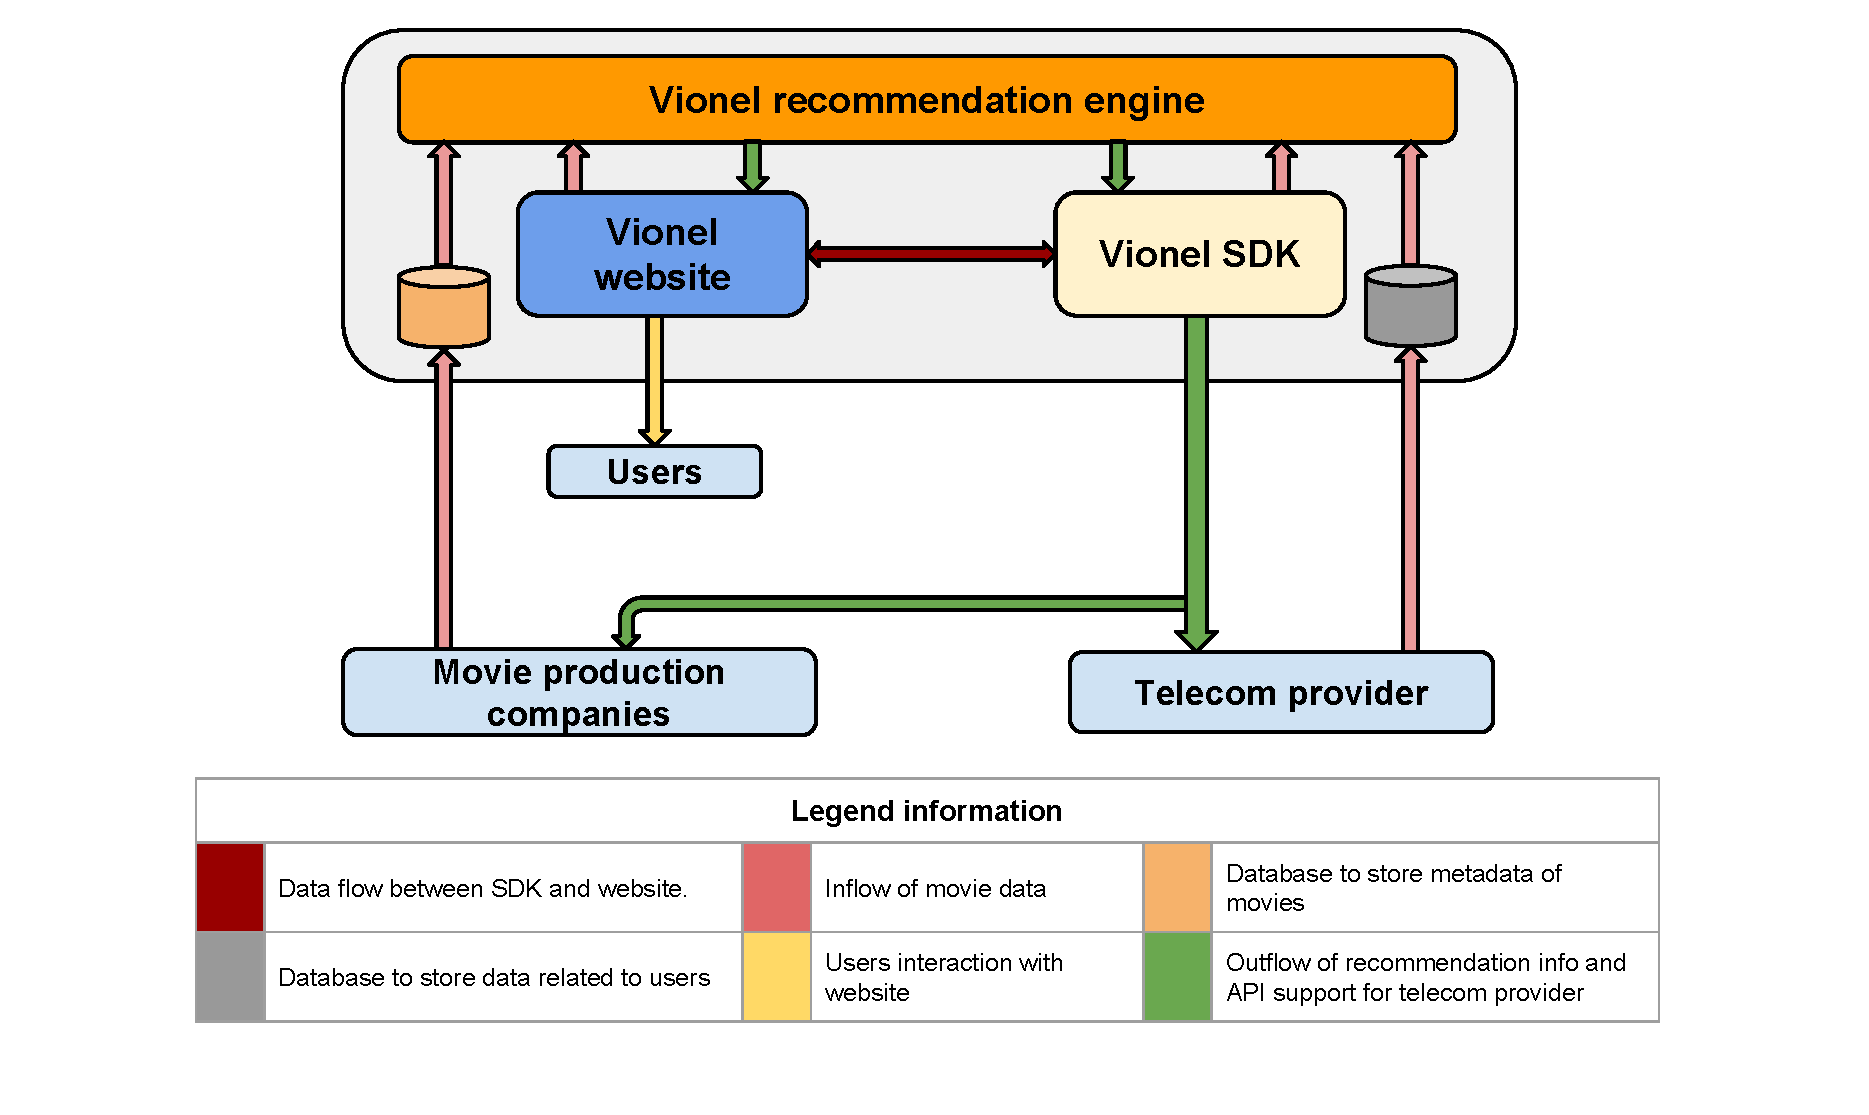
\includegraphics[scale=0.5]{Figures/Business_ecosystem.pdf}
		%\rule{35em}{0.5pt}
	\caption[Figure: Proposed business ecosystem]{Proposed business ecosystem, Source: Vion Labs marketing team}
	\label{fig: Proposed business ecosystem}
    \end{figure}  

 \subsection {Technical changes to increase uniqueness} 
  \label{Technical_changes_to_increase_uniqueness}
   % Spotify ,social media, innovative ratings (questionarie based), computer vision algos, hybrid recommender system. Where to watch ? , Mood based, voice based mood detection and movie suggestion, location based, time and day based, weather and mood based recommendations, surprises, mention about Jinni, how it used innovative solutions to gain competitive edge ...    
    As described in section \ref{Competitive_advantage_tech_differentiation} of literature study, the way of creating an good image in the minds of customers is by providing them with better valued product. In order to do so, there are changes required in the technical features of Vionel. The motto of web recommendation engines is to engage users by providing quality content and recommendations. To create technological differentiation of recommendations, several innovative ideas needs to be incorporated into architecture of recommendation systems. One such feature is to provide recommendations for a new user by solving the problem of cold start as described in section \ref{Buisness_related_changes} by developing Vionel software development kit to support inclusion of user's data as input to recommendation engine. The trend of recommendation engines is moving towards hybrid recommendation engines, where recommendations generated are combination of both content information and history data of user ratings. Vionel can benefit by adopting its technical architecture to support hybrid recommendations to its users. 

    Partnering with companies such as Spotify to get access to its customer data, in return providing space in website to publish songs related to movies. The quality of recommendations provided by Vionel can be further improved by getting access to songs liked by a user. Since, it is highly likely that a user liking a song from a movie, would like that movie or related movies. Overall, by using efficient user data analytics, a person's complete entertainment taste can be predicted accurately. On the other hand there is a possibility of getting access to user's personal data such as location, likes and dislikes info about a subject by respecting privacy of users, while partnering with social media companies. An ideal recommendation engine should provide suggestions to the user by recognizing user's mood at that instance, an effort in this lines has been considered by our competitor Jinni, which provides recommendations based on mood information selected by user. Other innovative features that could be used for the purpose of providing recommendations are based on user's location, time of the day, day of the week information and weather information, which influences mood of the users. 

    In a lateral dimension, computer vision algorithms combined with machine learning algorithms can be used to increase features that act as input to the recommender system. This involves movie content analysis to detect interesting features of movies like environment information, product placement information, color information, speed of the movie and others to generate large category of tags for movies. The feature of voice based navigation through website is an interesting feature to add, along with this a machine learning algorithm can be used to detect mood of a person based on voice information and it can be later used to recommend movies. A computer vision based method of detecting user's mood uses the technique of facial expression interpretation by capturing real time video feed. With this feature users who have little or no computer knowledge, especially elderly people will be able to use Vionel, with voice based navigation movie search feature. These innovative features will attract more number of users and also would encourage them to use our recommendation services before watching a movie.     

\section{Teams role in attaining competitive edge}
 % tech team , marketing team
 %R \& D team responsibility,  
    Achieving competitive sustainable advantage is a collective effort from all member teams of a company. The respective responsibilities that needs to taken by the teams are as follows:
    \begin{itemize}

    \item CEO and Marketing team members : 
    The role of marketing members is to find partners ranging from movie production franchises, movie content providers and companies that are willing to embed plug-ins (example: Spotify). In order to improve discovery of the website, actively participating in press related events, representing organization in business events, startup meets to attract investors. Finally, to create a sustainable business ecosystem where Vionel can thrive upon by inhibiting other competitors in the business and creating a powerful barrier for new entrants in movie recommendation business.  
    
    \item Research team members : 
    The main responsibility of adding innovative features by performing research to enhance the capabilities of recommendation engines is with research team members. Adopting high tech methods of research to develop and improve recommendation algorithm that supports multiple type of recommendations. Development of baseline recommender engine on top of baseline movie content discovery framework.
    
    \item Development and production unit team members : 
    Development team members ensure faster development of researched features and publish it in the website. Other responsibilities of team members involve ensuring faster response time, avoiding website downtime, developing user friendly web pages for the website, efficient handling of user data, and recommendation SDK development. 

    \item Personal relationship (PR) team members : 
    PR team members responsibility is to collect opinions from the users, answer queries related to website content, and also to receive customer complaints, suggestions regarding Vionel product. This information has to passed over to research team to facilitate addition of new feature into recommendation system.

    \end{itemize}  
       
\section{Contribution from internship work}
 % innovative feature for recommender systems
   The main contribution from the internship work is to enable automatic brand logo detections in movies. The process of detecting brand logos in movies is tough job for humans, hence internship effort was to perform the task of brand logo detection using computer vision algorithm combined with machine learning technique. One more important contribution was to reduce the time taken for extracting features from movies using cluster of graphical processing units. Currently brand logo detector can detect ten specific brands from movies to create tags for recommendation engine to improve its suggestions to users. A framework is created to include brand logos of other companies in future, to generate accurate tags from movies. There has been considerable reduction of processing time per movie by using computational power of GPUs. Currently the time taken for processing and generating tags has been halved with the use of two GPUs in parallel. Future projects can use the developed framework to parallelize extraction of features using machine learning techniques on videos. These contributions help R\&D team to innovate more by faster prototyping of ideas, it can also be used to generate more tags automatically from new movies that are added into the database. Reduction in time and addition of innovative tags increases technical differentiation from our competitors, thereby helping Vionel to achieve competitive edge in view of customers.        

\section{Conclusion}
 % How technological differentiation enables a company to attain competitive edge over other companies. Write about next step in innovation processes
   Comparative analysis of features supported by companies has increased knowledge about competition, also information about driving factors that enables a movie recommendation product to be popular have been critically accessed. Gained knowledge during the analysis could be used during next stage in the innovation process for \acrshort{MRS} product. Especially, the collected information helps in early identification, during ideation phase, the critical features that should be supported by Vionel to achieve success. A clear understanding of how technical differentiation of a product assists a company to achieve sustainable competitive advantage is characterized in the case of movie recommendation industry. Overall, this report takes one step further in innovation framework for recommendation engine product of Vion Labs. It provides valuable information of highly competitive companies in the market, which can be further used to determine competitive strategies to achieve sustainable competitive advantage by attracting and retaining more number of users.